\chapter{Monge 問題}
\label{ch:sem-monge-chapter}

定義~\ref{def:sem-assignment}は有限の添字集合 $\range{n}$ と
均一重み $1/n$ を扱う離散的な輸送問題だった．次の対応で一般の定義~\ref{def:sem-polish}
$\X, \Y$ と任意の確率測度（定義~\ref{def:sem-probability-measure}）に拡張する：
\begin{center}
  \begin{tabular}{l|ll}
    & 最適割当問題 & Monge 問題 \\ \hline
    source/target & $\range{n}$（重み $1/n$） & $\alpha \in \Mm_+^1(\X)$，$\beta \in \Mm_+^1(\Y)$ \\
    輸送写像 & 置換 $\sigma \in \Perm(n)$ & 可測写像 $T \colon \X \to \Y$ \\
    全射制約 & $\sigma$ が全単射 & 定義~\ref{def:sem-pushforward} $T\pushforward \alpha = \beta$ \\
    総コスト & $\frac{1}{n}\sum_i C_{i, \sigma(i)}$ & $\int_\X c(x, T(x))\, \d\alpha(x)$
  \end{tabular}
\end{center}
これに基づく連続版の輸送問題が \textbf{Monge 問題}である．

\begin{definition}{Monge 問題}{sem-monge}
\blockmeta{space=polish}
  $\X, \Y$ 上の確率測度（定義~\ref{def:sem-probability-measure}）$\alpha \in \Mm_+^1(\X)$, $\beta \in \Mm_+^1(\Y)$ と
  可測関数 $c \colon \X \times \Y \to \Rnn$ に対して，
  \textbf{Monge 問題}とは
  \[
    \inf_{T}
    \left\{
    \int_{\X} c(x, T(x)) \, \d\alpha(x)
    \;\middle|\;
    T \colon \X \to \Y \text{ は可測}, \;
    T\pushforward \alpha = \beta
    \right\}
  \]
  を求める問題である．ここで $T\pushforward \alpha$ は
  押し出し（定義~\ref{def:sem-pushforward}）を表す．
\end{definition}

$c(x, y)$ を $x$ から $y$ への\textbf{輸送コスト}と解釈すれば，
写像 $T \colon \X \to \Y$ は $x$ にある質量を $T(x)$ へ送ることを意味し，
目的関数 $\int_\X c(x, T(x)) \, \d\alpha(x)$ はその輸送の総コストを表す．
この問題には次節で示す通り，実行可能集合の \textbf{非凸性} と
\textbf{解の非存在}という本質的な困難があり，
\textbf{Kantorovich 緩和}はこれらをカップリングによって解消する．

%% --- Monge 問題のイメージ図 ---
\begin{figure}[htbp]
\centering
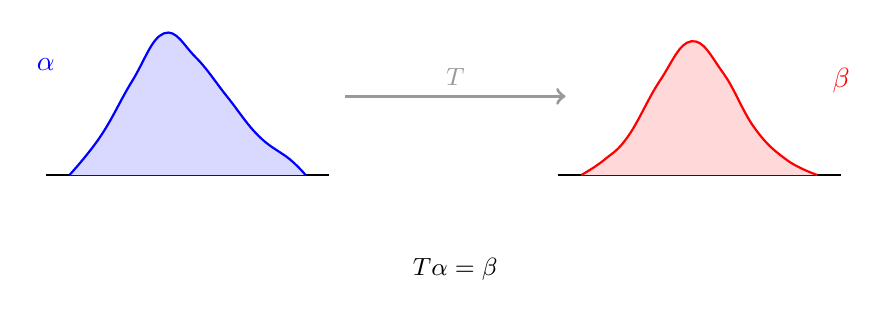
\begin{tikzpicture}[scale=1.0]
  % --- $\X$ と $\alpha$ ---
  \begin{scope}
    \draw[thick] (-0.3, 0) -- (3.3, 0);
    \node[below] at (1.5, -0.4) {$\X$};
    \fill[blue!15] plot[smooth, tension=0.7]
      coordinates {(0,0) (0.4,0.5) (0.8,1.2) (1.2,1.8) (1.6,1.5)
                   (2.0,1.0) (2.4,0.5) (2.8,0.2) (3.0,0)}
      -- cycle;
    \draw[thick, blue] plot[smooth, tension=0.7]
      coordinates {(0,0) (0.4,0.5) (0.8,1.2) (1.2,1.8) (1.6,1.5)
                   (2.0,1.0) (2.4,0.5) (2.8,0.2) (3.0,0)};
    \node[blue] at (-0.3, 1.4) {$\alpha$};
  \end{scope}

  % --- 写像 T ---
  \draw[->, very thick, gray!80] (3.5, 1.0) -- (6.3, 1.0)
    node[midway, above, font=\small] {$T$};

  % --- $\Y$ と $\beta$ ---
  \begin{scope}[xshift=6.5cm]
    \draw[thick] (-0.3, 0) -- (3.3, 0);
    \node[below] at (1.5, -0.4) {$\Y$};
    \fill[red!15] plot[smooth, tension=0.7]
      coordinates {(0,0) (0.3,0.2) (0.6,0.5) (1.0,1.2) (1.4,1.7)
                   (1.8,1.3) (2.2,0.6) (2.6,0.2) (3.0,0)}
      -- cycle;
    \draw[thick, red] plot[smooth, tension=0.7]
      coordinates {(0,0) (0.3,0.2) (0.6,0.5) (1.0,1.2) (1.4,1.7)
                   (1.8,1.3) (2.2,0.6) (2.6,0.2) (3.0,0)};
    \node[red] at (3.3, 1.2) {$\beta$};
  \end{scope}

  % --- 押し出し条件 ---
  \node[font=\small] at (4.9, -1.2)
    {$T\pushforward \alpha = \beta$};
\end{tikzpicture}
\caption{Monge 問題．$\X$ 上の分布 $\alpha$ が写像 $T$ で $\Y$ 上の分布 $\beta$ に押し出される．押し出しの詳細は命題~\ref{prop:sem-dirac-pushforward} 付近の略図を参照．}
\label{fig:sem-monge}
\end{figure}

\subsection{Monge 問題の本質的困難}

\subsubsection{困難1：実行可能集合の非凸性}

$\X = \Y = \R$ とする．
このとき可測写像 $T \colon \R \to \R$ の全体は，点ごとの和・スカラー倍
$(tT_1 + (1-t)T_2)(x) \defeq t\, T_1(x) + (1-t)\, T_2(x)$
によりベクトル空間をなす．この空間の部分集合としての
Monge 問題の実行可能集合
\[
  \mathcal{T}(\alpha, \beta)
  \defeq \left\{ T \colon \X \to \Y \;\middle|\;
  T \text{ は可測},\; T\pushforward \alpha = \beta \right\}
\]
は一般に凸（定義~\ref{def:sem-convex}）でない．

\begin{example}{実行可能集合の非凸性}{sem-nonconvex}
  $\alpha = \beta = \tfrac{1}{2}\delta_{-1} + \tfrac{1}{2}\delta_1$ とし，
  \[
    T_1(x) = x,\qquad T_2(x) = -x,\qquad t = \tfrac{1}{2}
  \]
  をとる．$\alpha$ の定義を代入し，命題~\ref{prop:sem-dirac-pushforward} (ii) を適用すると
  \begin{align*}
    {T_1}\pushforward \alpha
    &= {T_1}\pushforward \bigl(\tfrac{1}{2}\delta_{-1} + \tfrac{1}{2}\delta_{1}\bigr)
      && \text{（$\alpha$ の定義）} \\
    &= \tfrac{1}{2}\delta_{T_1(-1)} + \tfrac{1}{2}\delta_{T_1(1)}
      && \text{（命題~\ref{prop:sem-dirac-pushforward} (ii)）} \\
    &= \tfrac{1}{2}\delta_{-1} + \tfrac{1}{2}\delta_{1} = \beta
      && \text{（$T_1(x) = x$ より）}.
  \end{align*}
  同様に
  \begin{align*}
    {T_2}\pushforward \alpha
    &= {T_2}\pushforward \bigl(\tfrac{1}{2}\delta_{-1} + \tfrac{1}{2}\delta_{1}\bigr)
      && \text{（$\alpha$ の定義）} \\
    &= \tfrac{1}{2}\delta_{T_2(-1)} + \tfrac{1}{2}\delta_{T_2(1)}
      && \text{（命題~\ref{prop:sem-dirac-pushforward} (ii)）} \\
    &= \tfrac{1}{2}\delta_{1} + \tfrac{1}{2}\delta_{-1} = \beta
      && \text{（$T_2(x) = -x$ より $T_2(-1) = 1,\, T_2(1) = -1$）}.
  \end{align*}
  よって $T_1, T_2 \in \mathcal{T}(\alpha, \beta)$ である．

  一方，$\bar{T} = \tfrac{1}{2}T_1 + \tfrac{1}{2}T_2$ は
  $\bar{T}(x) = \tfrac{1}{2}x + \tfrac{1}{2}(-x) = 0$
  すなわち $0$ を値にとる定値写像であり，
  $\bar{T}\pushforward\alpha = \delta_0 \neq \beta$．
  よって $\bar{T} \notin \mathcal{T}(\alpha, \beta)$ であり，
  $\mathcal{T}(\alpha, \beta)$ は凸でない．
\end{example}

\subsubsection{困難2：解の非存在}

\begin{example}{Monge 写像が存在しない場合}{sem-monge-noexist}
  $\alpha = \delta_0$（質量 $1$ が 1 点 $0$ に集中）と
  $\beta = \tfrac{1}{2}\delta_{-1} + \tfrac{1}{2}\delta_1$（2 点に質量 $\tfrac{1}{2}$ ずつ分散）
  を考える．任意の可測写像 $T \colon \R \to \R$ について
  命題~\ref{prop:sem-dirac-pushforward} (i) より
  \[
    T\pushforward \alpha = T\pushforward \delta_0 = \delta_{T(0)}
  \]
  となる．これは点 $T(0)$ に質量 $1$ を集中させた測度ゆえ
  $\delta_{T(0)}(\{T(0)\}) = 1$．一方 $\beta$ は任意の単点 $\{y\}$ に対し
  $\beta(\{y\}) \in \{0,\, \tfrac{1}{2}\}$（$y = \pm 1$ のとき $\tfrac{1}{2}$，
  それ以外で $0$）しか与えないので，どの $T(0) \in \R$ をとっても
  $\delta_{T(0)} \neq \beta$ である．
  したがって $T\pushforward \alpha = \beta$ をみたす $T$ は存在せず，
  $\mathcal{T}(\alpha, \beta) = \emptyset$（下図）．

  \begin{center}
  \begin{tikzpicture}[scale=1.0]
    \draw[->] (-1.8, 0) -- (1.8, 0);
    \draw[thick, blue] (0, 0) -- (0, 1.2);
    \fill[blue] (0, 1.2) circle (2pt);
    \node[below] at (0, -0.1) {$0$};
    \node[above, blue] at (0, 1.35) {$\alpha = \delta_0$};

    \draw[->, thick, dashed, gray] (2.2, 0.6) -- (3.2, 0.6);
    \node[above, gray] at (2.7, 0.6) {$T\, ?$};

    \begin{scope}[xshift=5cm]
      \draw[->] (-1.8, 0) -- (1.8, 0);
      \draw[thick, red] (-1, 0) -- (-1, 0.6);
      \fill[red] (-1, 0.6) circle (2pt);
      \draw[thick, red] (1, 0) -- (1, 0.6);
      \fill[red] (1, 0.6) circle (2pt);
      \node[below] at (-1, -0.1) {$-1$};
      \node[below] at (1, -0.1) {$1$};
      \node[above, red] at (0, 0.8) {$\beta = \tfrac{1}{2}\delta_{-1} + \tfrac{1}{2}\delta_1$};
    \end{scope}
  \end{tikzpicture}
  \end{center}
\end{example}
